%
% LaTeX Report Assignment 4
% Applied Programming Lab EE2703
% Ayush Jamdar EE20B018 
%


\documentclass[11pt, a4paper]{article}
\usepackage{graphicx}
\usepackage{amsmath}
\usepackage{listings}
\usepackage[]{courier}
%\usepackage{hyperref}


\title{EE2703: Endsemester Exam}

\author{Ayush Jamdar EE20B018} % Author name

\date{\today} % Date for the report
\begin{document}		
		
\maketitle % Insert the title, author and date
\section{Aim}
The goal is to study the distribution of currents in a dipole antenna and refresh Python concepts at the same time. From EE2025 I recall that the current distribution in this antenna is sinusoidal with zero current at the antenna ends. 
$$I = Im\sin(k(l-|z|))$$
where $-l<z<l$. $l$ is the antenna half-length ($\lambda = 4l$, here.). 
The question this assignment asks is how correct is this sinusoidal current assumption? Or is it exactly what happens in an antenna? Lets explore it using scientific methods of computation in Python.

\begin{figure}[!tbh]
   	\centering
  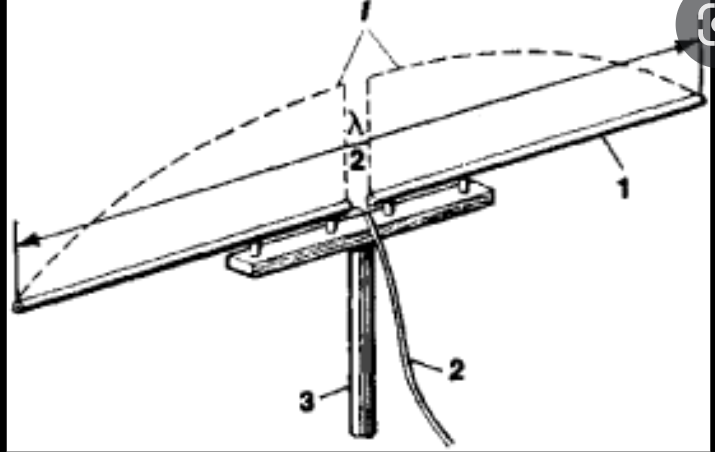
\includegraphics[scale=0.5]{antenna.png} 
    \caption{The Half Wavelength Dipole Antenna} 	
\end{figure}  

\subsection{The Assumed Current}
Some initial constants required, l = 50 cm, N = 4 sections, a = 0.01 radius of wire in m. Based on the above mentioned sinusoidal current variation, lets get this distribution in code. For this, we split the antenna into 2N+1 sections such that each half has N sections and the middle antenna feed is taken to be another.
$-l$ to $l$ is indexed in the \texttt{z} array. It is known that there is no current at the endpoints and it is Im at the center. This is done by the following lines of code:
\begin{verbatim}
z = np.linspace(-l, l, 2 * N + 1)
u = np.concatenate((z[1:N], z[N + 1 : 2 * N]))
I = Im * np.sin((2 * np.pi / lambda_) * (l - abs(z)))
  # current vector
J = np.concatenate((I[1:N], I[N + 1 : 2 * N]))
  # current vector J

\end{verbatim}
The result is printed out:
\begin{verbatim}
I_assumed =  [0.   0.38 0.71 0.92 1.   0.92 0.71 0.38 0.  ]
J_assumed =  [0.38 0.71 0.92 0.92 0.71 0.38] 
\end{verbatim}
Note that I is the current at each point in the z array but J has the currents at points except those specified by the boundary conditions.

\subsection{The Ampere's Law}
$$2\pi aH_{\phi}(z_{i}, r=a)=I_{i}$$
In a matrix form, it becomes 
$$H_{\phi}[z_{i}]=\frac{1}{2\pi a}I_{2N-2}J_i$$
I am tasked to create a function that creates this diagonal matrix. Here's how:
\begin{verbatim}
def find_M(size=2 * N - 2):
    return np.identity(size) / (2 * np.pi * a)
\end{verbatim}

\subsection{The Vector Potential}
$$A(r,z) = \frac{\mu_0}{4\pi}\int \frac{I(z)e^{-jkR}\hat{z}dz}{R}$$
$$A_{z,i}=\Sigma I_j(\frac{\mu_0e^{-jkR_{ij}}dz}{R_{ij}})$$
$$A_{z, i} = \Sigma P_{ij}I_j+P_BI_N$$
P is a matrix with 2N-2 columns and 2N-2 rows. PB is the contribution to the vector potential due to the current $I_N$. $R_z$ and $R_u$ are the distances from the observer at $\vec{r}+z_i\hat{z}$ and source at $z_j\hat{z}$. The difference between Rz and Ru is that the former computes distances to known currents and Ru is a vector of distances to unknown currents. I first compute $R_{zij} = \sqrt{a^2+(z_i-z_j)^2}$. Rz is a matrix of dimensions 2N+1 The below lines are an important vectorized code. Here, a matrix built out of recurring \texttt{z} as its rows and another as its columns. I subtract those two to get the latter half of the $R_{zij}$ equation. 

\begin{verbatim}
Rz = np.sqrt(
    (np.ones((2 * N + 1, 2 * N + 1)) * a) ** 2
    + (np.array([z] * (2 * N + 1)) - np.array([z] * 
    (2 * N + 1)).T) ** 2
)
\end{verbatim}   

A similar procedure on the \texttt{u} array gives Ru. Note that Ru is a square matrix of dimensions 2N-2. Also, the $R_{ij}$ used in $P_{ij}$ is this Ru.
\begin{verbatim}
Ru = np.sqrt(
    (np.ones((2 * N - 2, 2 * N - 2)) * a) ** 2
    + (np.array([u] * (2 * N - 2)) - np.array
    ([u] * (2 * N - 2)).T) ** 2
)
\end{verbatim}

The next step is computing $P_ij$. And Pb,$$P_B = \frac{\mu_0exp(-jkR_{iN})}{4\pi R_{iN}}$$ is the contribution due to $I_N$. Here I use \texttt{RiN} a column vector, which is built out of slices of Rz such that it gives 2N-2 elements (excluding boundaries). 
 
\begin{verbatim}
Pij = (mu0 / (4 * np.pi) * np.exp(-complex(0, k) * Ru)
 * dz) / (Ru)

RiN = np.concatenate(((Rz[:, N])[1:N], (Rz[:, N])
  [N + 1 : 2 * N]))
# Dimensions of RiN: 2N-2 x 1; See equations

Pb = (mu0 / (4 * np.pi)) * np.exp(-1j * (k * RiN)) * dz / RiN

\end{verbatim} 

These are the results I obtained.
\begin{verbatim}
Rz =  [[0.01 0.13 0.25 0.38 0.5  0.63 0.75 0.88 1.  ]
 [0.13 0.01 0.13 0.25 0.38 0.5  0.63 0.75 0.88]
 [0.25 0.13 0.01 0.13 0.25 0.38 0.5  0.63 0.75]
 [0.38 0.25 0.13 0.01 0.13 0.25 0.38 0.5  0.63]
 [0.5  0.38 0.25 0.13 0.01 0.13 0.25 0.38 0.5 ]
 [0.63 0.5  0.38 0.25 0.13 0.01 0.13 0.25 0.38]
 [0.75 0.63 0.5  0.38 0.25 0.13 0.01 0.13 0.25]
 [0.88 0.75 0.63 0.5  0.38 0.25 0.13 0.01 0.13]
 [1.   0.88 0.75 0.63 0.5  0.38 0.25 0.13 0.01]]
 
Ru =  [[0.01 0.13 0.25 0.5  0.63 0.75]
 [0.13 0.01 0.13 0.38 0.5  0.63]
 [0.25 0.13 0.01 0.25 0.38 0.5 ]
 [0.5  0.38 0.25 0.01 0.13 0.25]
 [0.63 0.5  0.38 0.13 0.01 0.13]
 [0.75 0.63 0.5  0.25 0.13 0.01]]
 
Pij*1e8 =  [[124.94-3.93j   9.2 -3.83j   3.53-3.53j  -0.  -2.5j
   -0.77-1.85j   -1.18-1.18j]
 [  9.2 -3.83j 124.94-3.93j   9.2 -3.83j   1.27-3.08j  -0.  -2.5j
   -0.77-1.85j]
 [  3.53-3.53j   9.2 -3.83j 124.94-3.93j   3.53-3.53j   1.27-3.08j
   -0.  -2.5j ]
 [ -0.  -2.5j    1.27-3.08j   3.53-3.53j 124.94-3.93j   9.2 -3.83j
    3.53-3.53j]
 [ -0.77-1.85j  -0.  -2.5j    1.27-3.08j   9.2 -3.83j 124.94-3.93j
    9.2 -3.83j]
 [ -1.18-1.18j  -0.77-1.85j  -0.  -2.5j    3.53-3.53j   9.2 -3.83j
  124.94-3.93j]]
  
Pb*1e8 =  [1.27-3.08j 3.53-3.53j 9.2 -3.83j
  9.2 -3.83j 3.53-3.53j 1.27-3.08j]
\end{verbatim}
\begin{align*}
    H_\phi(r, z_i) & = -\sum_{j} \frac{dz^{'}_j}{4\pi}(\frac{-jk}{R_{ij}}-\frac{1}{R^2_{ij}})\exp(-jkR_{ij})\frac{rI_j}{R_{ij}}                                \\
                   & = -\sum_{j}P_{ij}\frac{r}{\mu0}(\frac{-jk}{R_{ij}}-\frac{1}{R^2_{ij}})I_j + P_{B}\frac{r}{\mu0}(\frac{-jk}{R_{iN}}-\frac{1}{R^2_{iN}})I_m \\
                   & = \sum_{j}Q^{'}_{ij}I_j                                                                                                                   \\
                   & = \sum_{j}Q_{ij}I_{j} + Q_{Bi}Im
\end{align*}

From here I get the equations for $Q_{ij}$ and $Q_B$.

\begin{verbatim}
Qij = -Pij * (a / mu0) * (complex(0, -k) / Ru - 1 / Ru**2)
Qb = -Pb * a / mu0 * ((-1j * k) / RiN - 1 / (RiN**2))

\end{verbatim}

This is what I got.

\begin{verbatim}
Qij =  [[9.952e+01-0.j 5.000e-02-0.j 
   1.000e-02-0.j 0.000e+00-0.j 0.000e+00-0.j  0.000e+00-0.j]
 [5.000e-02-0.j 9.952e+01-0.j 5.000e-02-0.j 
   0.000e+00-0.j 0.000e+00-0.j  0.000e+00-0.j]
 [1.000e-02-0.j 5.000e-02-0.j 9.952e+01-0.j 
   1.000e-02-0.j 0.000e+00-0.j  0.000e+00-0.j]
 [0.000e+00-0.j 0.000e+00-0.j 1.000e-02-0.j 
   9.952e+01-0.j 5.000e-02-0.j  1.000e-02-0.j]
 [0.000e+00-0.j 0.000e+00-0.j 0.000e+00-0.j 
   5.000e-02-0.j 9.952e+01-0.j  5.000e-02-0.j]
 [0.000e+00-0.j 0.000e+00-0.j 0.000e+00-0.j 
   1.000e-02-0.j 5.000e-02-0.j  9.952e+01-0.j]]
  
Qb =  [0.  -0.j 0.01-0.j 0.05-0.j 0.05-0.j 
  0.01-0.j 0.  -0.j]
\end{verbatim}

\subsection{Final Current Computation}
The equation we have finally is
$$(M-Q)J=Q_BI_m$$
To find J, matrix inverse is the way.

\begin{verbatim}
J_calculated = np.dot(np.linalg.inv(find_M(2 * N - 2)
   - Qij), Qb * Im)
I_calculated = np.concatenate(
    ([0], np.concatenate((J_calculated[: N - 1],
       [Im], J_calculated[N - 1 :])), [0])
)
\end{verbatim}

The result I obtained:
\begin{verbatim}
I_calculated =  [ 0.e+00+0.j -0.e+00+0.j -1.e-04+0.j
 -6.e-04+0.j  1.e+00+0.j -6.e-04+0.j
 -1.e-04+0.j -0.e+00+0.j  0.e+00+0.j]
 
J_calculated =  [-0.    +0.j -0.0001+0.j -0.0006+0.j
 -0.0006+0.j -0.0001+0.j -0.    +0.j]
\end{verbatim}

Finally I plot the computed and assumed currents together to get the plot in Figure 1 for N=4 and Figure 2 for N=6.
\begin{figure}[!tbh]
   	\centering
  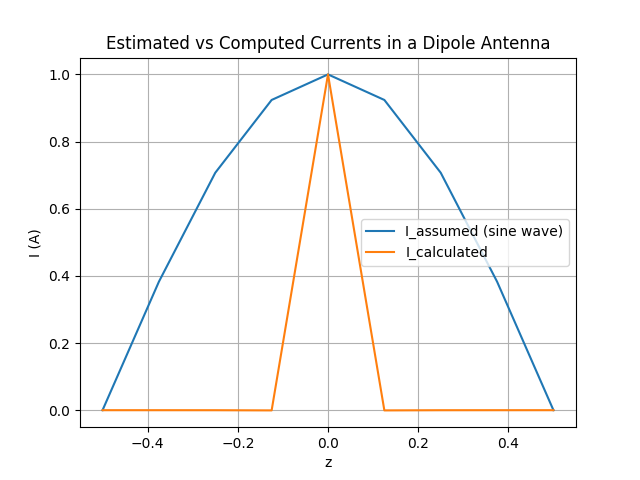
\includegraphics[scale=0.5]{f1.png} 
    \caption{N=4} 	
\end{figure}  

\begin{figure}[!tbh]
   	\centering
  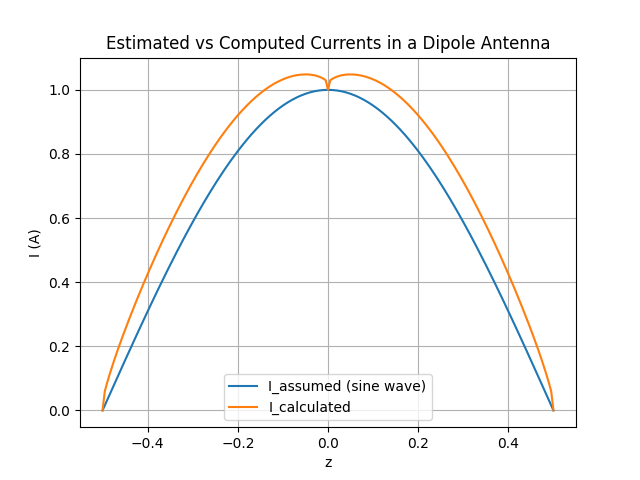
\includegraphics[scale=0.5]{f2.png} 
    \caption{N=100} 	
\end{figure}  

\section{Conclusion}
The aim that we took at the beginning of this assignment is now seen to have been accomplished. 
\end{document}